%
% Extension
% Abschlussarbeit (Bachelor)
%
% Thema: Erstellung einer Browser Extension zur Usability Evaluierung von beliebigen Web-Applikationen über Heatmaps.
% Betreuer 1: Prof. Dr. Targo Pavlista
% Betreuer 2: Siamak Haschemi
%
% @author Christian Bromann <contact@christian-bromann.com>
%

\section{Extension}

Für die Durchführung der Tests und der Aufzeichnung der Daten ist die Chrome Extension verantwortlich. Sie muss bei jedem Probanden installiert sein, um am Test teilzunehmen. Dies ist sicherlich zu erst einmal hinderlich, da zum Einen nicht zu erwarten ist, dass ein Testuser diese Extension nutzen möchte, und zum Anderen, dass dieser auch einen Chrome Browser bei sich auf dem System installiert hat. Dennoch ermöglicht es den Nutzern von \textit{thEvaluator}, Testcases für jede beliebige Webseite zu erstellen und aus den Nutzerverhalten dieser zu lernen. Es ist ein Alleinstellungsmerkmal, welches am Ende Vorteile gegenüber Konkurrenzprodukten bringen kann.\\
\\
Da sich die Extension zum Zeitpunkt der Abgabe dieser immer noch in einer Art Beta-Phase befindet, wird auf die Einbindung in den Google Web Store\footnote{\url{https://chrome.google.com/webstore}} verzichtet. Für den Beta-Test konnten sich die Probanden die Extension auf der offiziellen Projektwebsite\footnote{\url{http://qcentral.org/}} herunterladen. Da Google es verbietet fremde Extension mit einem einfachen Klick in den Browser einzubinden, muss diese erst heruntergeladen werden und via Drag\&Drop auf die Extensionseite\footnote{\url{chrome://extensions/}} des Browsers gezogen werden. Erst dann wird die Installation von Store-fremden Extensions gestattet. Ist dies erledigt erscheint in der Extension-Bar des Chrome Browsers ein kleines bunten Icon der \textit{thEvaluator}-Erweiterung. Klickt man darauf, so öffnet sich diese in einem kleinen Fenster. Zu sehen ist eine kleine Erläuterung zum Vorgehen des Testes und eine Textbox, wo die Testcase-ID eingegeben werden muss.

\begin{center}
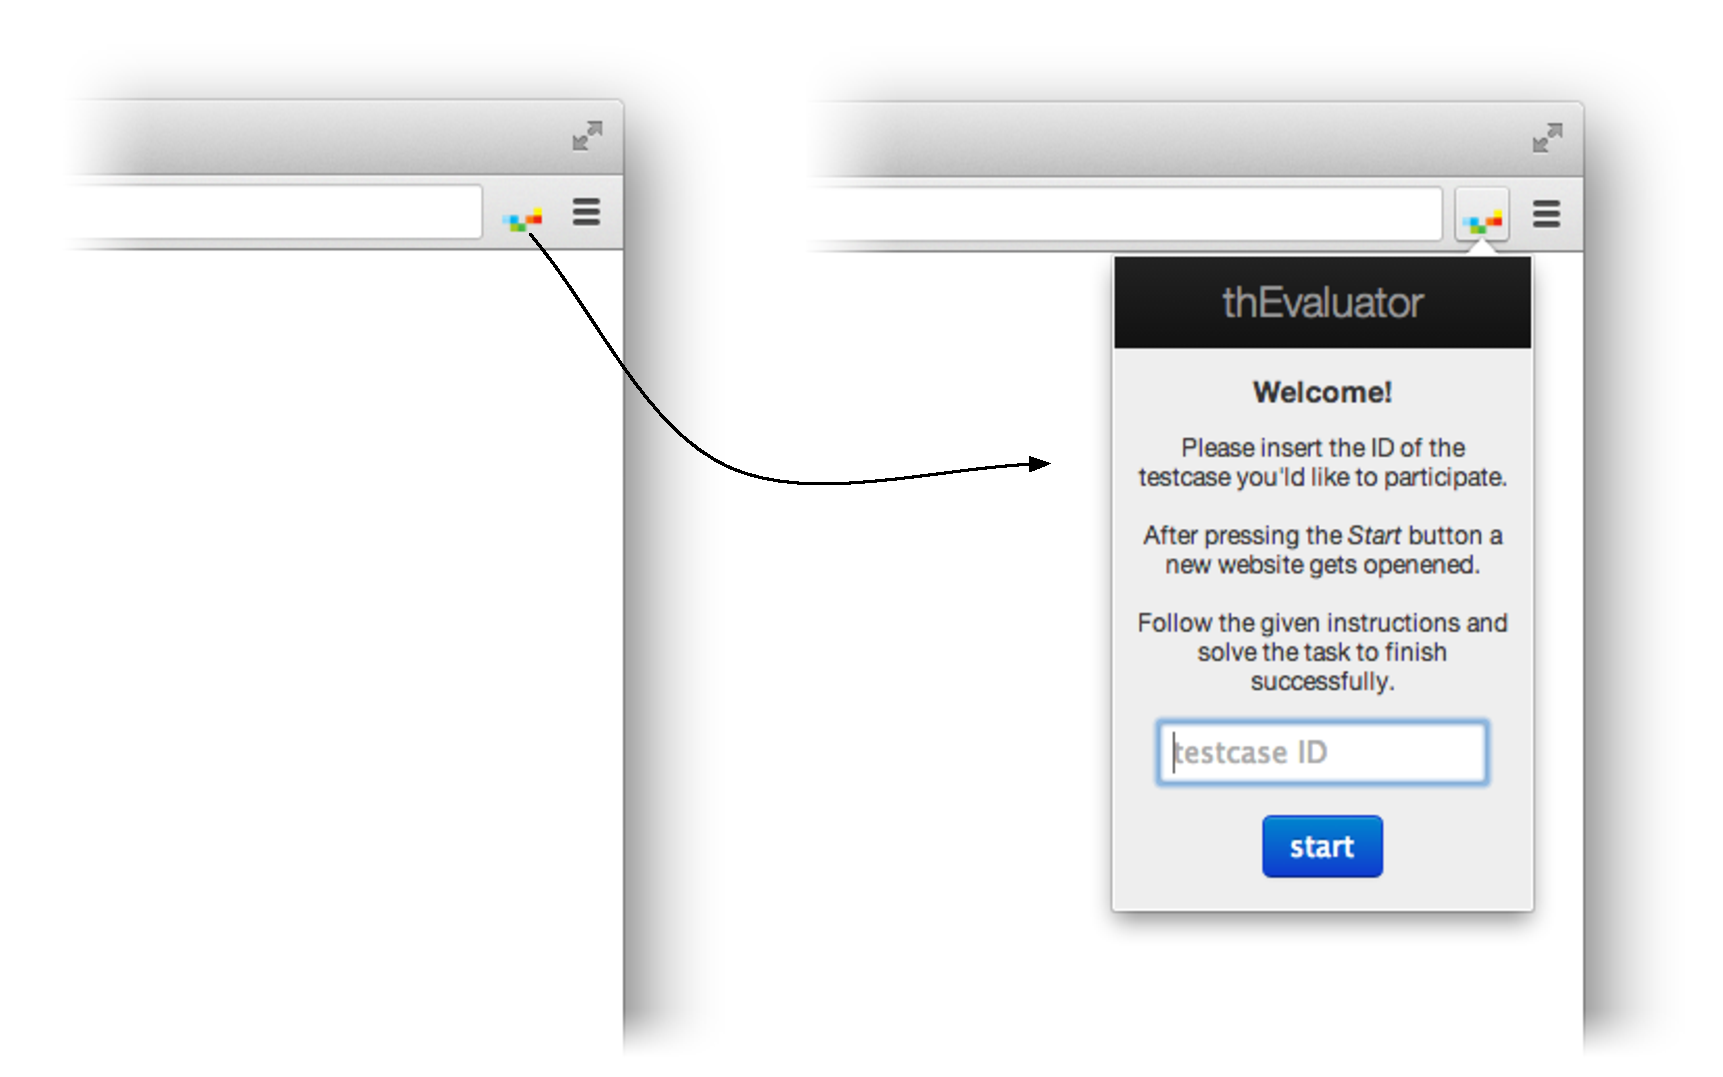
\includegraphics[scale=0.55]{./images/extension}
\end{center}
\begin{figure}[htb]
   \centering
   \caption{Aussehen der \textit{thEvaluator} Extension im Chrome Browser\\nach der Installation}
    \label{extension}
\end{figure}

Sobald der Proband die 10-stellige ID eingegeben hat und den \textit{start} Button drückt, beginnt der Testlauf. Die Extension öffnet dann einen neuen Tab und leitet den User auf die Start-URL.

\subsection{Aufbau}

Die Inhaltsstoffe einer Chrome Extension sind ganz normale HTML, CSS und JavaScript Dateien. Zusammengehalten wird alles durch ein Manifest, welches die Inhaltsstoffe auflistet und Rechte und Restriktionen festlegt. Jeder Nutzer bekommt bei der Installation angezeigt, welche diese sind und kann entscheiden, ob er sie zulassen möchte.
\\
\begin{lstlisting}[caption=Auszug aus der Manifest.json der \textit{thEvaluator} Extension,label=manifest]
{
    "manifest_version": 2,
    "name": "thEvaluator",
    "version": "0.1",
    "description": "Chrome extension to start thEvaluator usability tests",
    "browser_action":   {
        "default_icon": "img/icon128.png",
        "default_popup": "index.html"
    },
    "icons": { 
        "16": "img/icon16.png",
        "...": "..."
    },
    "background": {
        "page": "background.html"
    },
    "permissions": [ "cookies", "tabs", "http://*/*", "https://*/*" ],
    "content_scripts": [{
        "js": [
            "js/thEvaluatorWidget.js",
            "..."
        ],
        "css": ["dist/injected.css"],
        "all_frames": true
    }],
    "web_accessible_resources": [
        "templates/task.tpl",
        "..."
    ]
}
\end{lstlisting}

Listing \ref{manifest} zeigt einen Auszug des Manifestes der \textit{thEvaluator} Chrome Extension. Neben Name, Versionsnummer und Beschreibung der Extension werden zusätzlich Icons bestimmt und die Rolle der einzelnen HTML Seiten festgelegt.\\
\\
Eine weitere Komponente der Extension sind die Grunt\footnote{\url{http://gruntjs.com/}} Tasks. Diese kümmern sich um das Testen und Kompilieren der Extension zu einem Paket und die anschließende Umwandlung zu einer Chrome Extension Datei mit der Endung \textit{.crx}. Grunt ist ein Task-Manager, basierend auf NodeJS, welcher durch Plugins erweitert werden kann und die Entwicklung von Web-Applikationen jeglicher Art automatisiert. Die Tasks werden dabei in einer zentralen Datei, dem Gruntfile, definiert und können jeder Zeit über die Konsole ausgeführt werden. Durch die Kompilierung der Extension durch Grunt werden die CSS und JavaScript Dateien zusammengefügt und minifiziert. Dadurch schrumpft die Dateigröße der Erweiterung und macht den Sourcecode unlesbar.

\subsection{Architektur}
% http://developer.chrome.com/extensions/overview.html

\subsection{Nachrichtenübermittlung}
% http://developer.chrome.com/extensions/messaging.html

\subsection{Datenaufzeichnung}
% Welche Daten werden wann aufgezeichnet
% Screenshot Erstellung
% Problematik der erhšöhten Datenmenge